%LTeX: language=it
\subsection{UC 4 - Creazione di un contatto} \label{sec:UC4}
    \begin{itemize}
        \item \textbf{Attore principale}: MUA;
        \item \textbf{Descrizione}: il MUA crea un contatto nel sistema;
        \item \textbf{Precondizioni}: il MUA sta usando la funzionalità di creazione di un oggetto;
        \item \textbf{Postcondizioni}: il sistema salva il contatto con le informazioni fornite dal MUA;
        \item \textbf{Scenario principale}:
            \begin{enumerate}
                \item il MUA invia i dettagli del contatto al sistema (\hyperref[sec:UC4.1]{UC 4.1});
                \item il sistema salva il contatto;
            \end{enumerate}
        \item \textbf{Inclusioni}: nessuna;
        \item \textbf{Generalizzazioni}: nessuna;
        \item \textbf{Estensioni}: nessuna.
    \end{itemize}

\begin{figure}[h]
    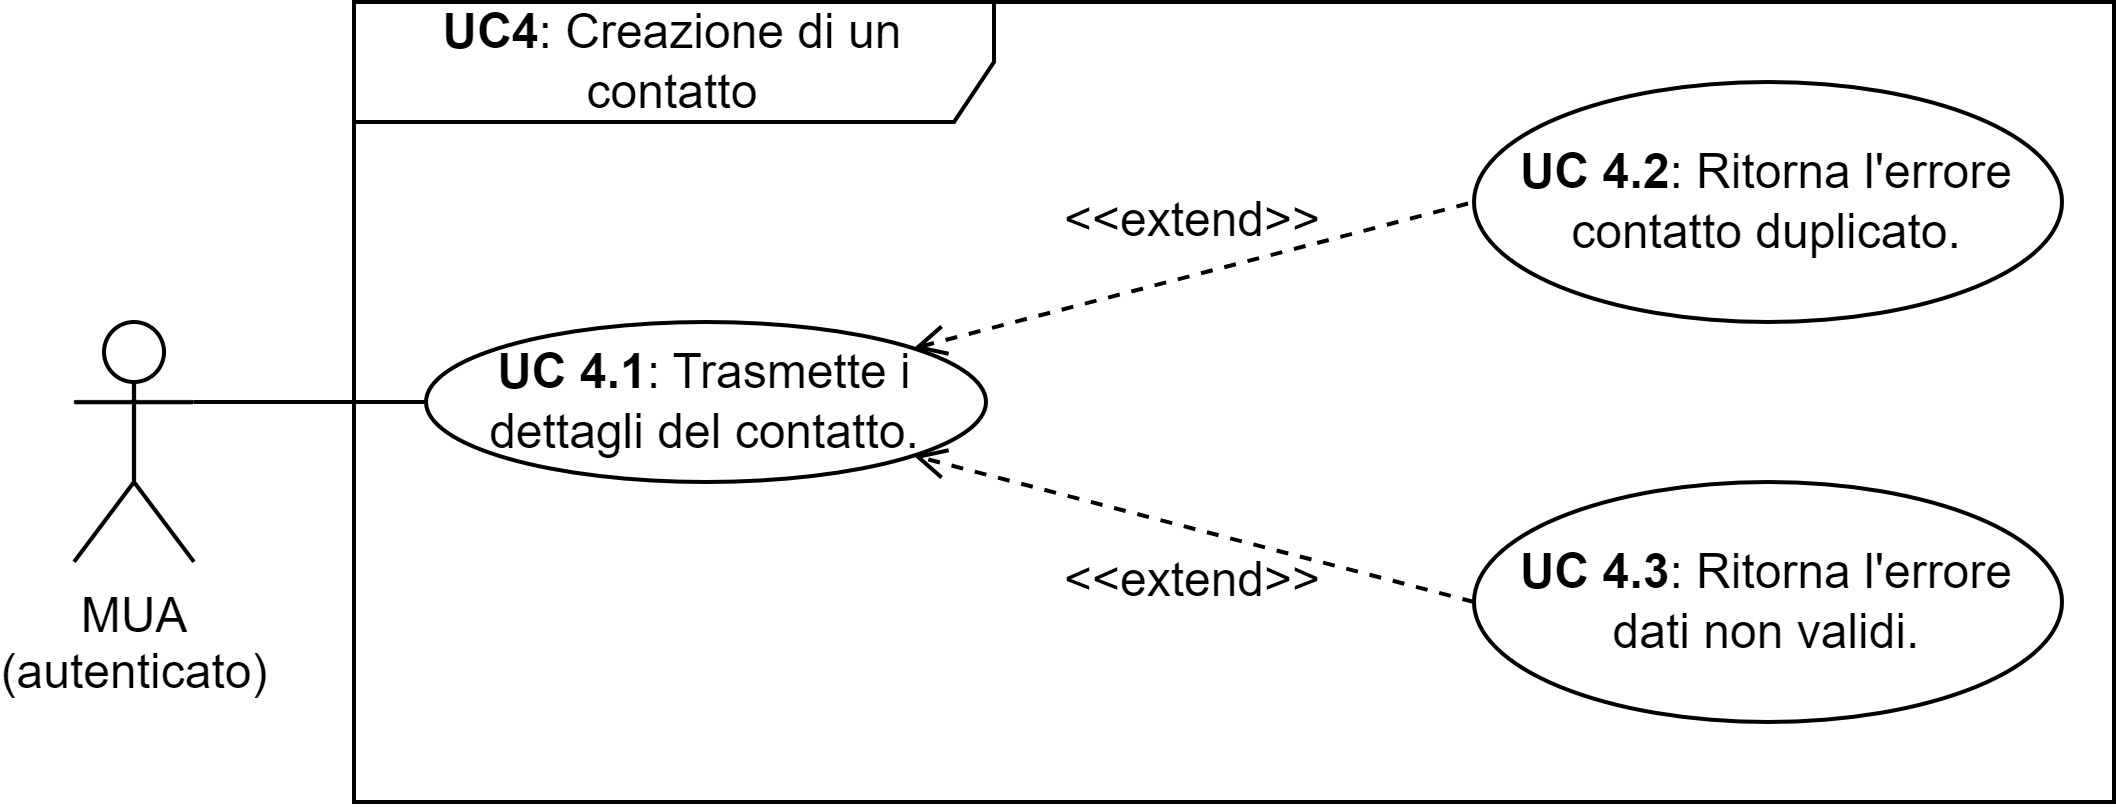
\includegraphics[width=0.85\textwidth]{sections/uc_imgs/UC04.X.png}
    \centering
    \caption{Diagramma sotto-casi UC 4.}
\end{figure}

\subsubsection{UC 4.1 - Trasmette i dettagli del contatto} \label{sec:UC4.1}
    \begin{itemize}
        \item \textbf{Attore principale}: MUA;
        \item \textbf{Descrizione}: il MUA invia le informazioni del contatto al sistema;
        \item \textbf{Precondizioni}: il MUA sta usando la funzionalità di creazione di un contatto;
        \item \textbf{Postcondizioni}: il sistema salva il contatto con le informazioni fornite dal MUA;
        \item \textbf{Scenario principale}:
            \begin{enumerate}
                \item il MUA invia i dettagli del contatto al sistema;
                \item il sistema controlla che le informazioni ricevute rispettino il seguente requisito minimo:
                    \begin{itemize}
                        \item il nome del contatto non è vuoto;
                    \end{itemize}
            \end{enumerate}
        \item \textbf{Inclusioni}: nessuna;
        \item \textbf{Generalizzazioni}: nessuna;
        \item \textbf{Estensioni}:
            \begin{enumerate}[label=\alph*.]
                \item il sistema non riesce a salvare il contatto perché è un duplicato:
                \begin{enumerate}[label=\arabic*.]
                    \item il sistema ritorna un errore al MUA di contatto duplicato (\hyperref[sec:UC4.2]{UC 4.2});
                \end{enumerate}
                \item il sistema non riesce a salvare il contatto perché è un duplicato:
                \begin{enumerate}[label=\arabic*.]
                    \item il sistema ritorna un errore al MUA perché le informazioni del contatto non rispettano i requisiti (\hyperref[sec:UC4.3]{UC 4.3}).
                \end{enumerate}
            \end{enumerate}
    \end{itemize}


\subsubsection{UC 4.2 - Ricezione errore contatto duplicato} \label{sec:UC4.2}
    \begin{itemize}
        \item \textbf{Attore principale}: MUA;
        \item \textbf{Descrizione}: il sistema non riesce a salvare il contatto perché esiste già nella rubrica;
        \item \textbf{Precondizioni}: il MUA sta usando la funzionalità d'invio dei dettagli al sistema di un contatto;
        \item \textbf{Postcondizioni}: il sistema non salva il nuovo contatto, il MUA è stato notificato dell'errore;
        \item \textbf{Scenario principale}:
            \begin{enumerate}
                \item il sistema riscontra che il contatto già esiste;
                \item il sistema non salva il contatto e notifica il MUA dell'errore;
            \end{enumerate}
        \item \textbf{Inclusioni}: nessuna;
        \item \textbf{Generalizzazioni}: nessuna;
        \item \textbf{Estensioni}: nessuna.
    \end{itemize}

\subsubsection{UC 4.3 - Ricezione errore dettagli contatto non validi} \label{sec:UC4.3}
    \begin{itemize}
        \item \textbf{Attore principale}: MUA;
        \item \textbf{Descrizione}: il sistema non riesce a salvare il contatto perché i dettagli del contatto non rispettano i requisiti;
        \item \textbf{Precondizioni}: il MUA sta usando la funzionalità d'invio dei dettagli al sistema di un contatto;
        \item \textbf{Postcondizioni}: il sistema non salva il nuovo contatto, il MUA è stato notificato dell'errore;
        \item \textbf{Scenario principale}:
            \begin{enumerate}
                \item il sistema riscontra i dettagli del contatto ricevuti dal MUA non rispettano i requisiti mini;
                \item il sistema non salva il contatto e notifica il MUA dell'errore;
            \end{enumerate}
        \item \textbf{Inclusioni}: nessuna;
        \item \textbf{Generalizzazioni}: nessuna;
        \item \textbf{Estensioni}: nessuna.
    \end{itemize}